\documentclass[a4paper,14pt]{extarticle}

\usepackage[top=1in, bottom=1in, left=1in, right=1in]{geometry}
\usepackage[utf8]{inputenc}
\usepackage[russian]{babel}
\usepackage{graphicx}
\usepackage{caption}
\usepackage{subcaption}
\usepackage{chngcntr}
\usepackage{amsmath}
\usepackage{amsfonts}
\usepackage{pgfplots}
\usepackage{pgfplotstable}
\usepgfplotslibrary{fillbetween}
\usepackage{float}
\usepackage{lipsum}% http://ctan.org/pkg/lipsum
\usepackage{multicol}% http://ctan.org/pkg/multicol
\usepackage{hhline}
\usepackage{tabularx}
\usepackage{tikz,xcolor}
\usepackage{tkz-graph}
\usepackage{float}
\usepackage{mathtools}
\usepackage{todonotes}
\usepackage{listings}
\usepackage[makeroom]{cancel}

\usetikzlibrary{arrows, petri, topaths}

\counterwithin{figure}{section}
\counterwithin{equation}{section}
\counterwithin{table}{section}

\begin{document}
\begin{titlepage}
\centering 
{\bfseries Санкт-Петербургский Политехнический Университет} \\
Институт компьютерных наук и технологий \\
Кафедра компьютерных систем и программных технологий \\
\vspace{5cm}
{\centering \textbf{Отчёт о лабораторной работе 7} \\ 
\vspace{0.2cm}
\textbf{Дисциплина}: Телекоммуникационные технологии \\
\vspace{0.2cm}
\textbf{Тема}: Помехоустойчивые коды. } \\
\vspace{4cm}
\hfill {\bfseries Работу выполнил:}  \\
\hfill гр. 33501/3 Кнорре А.В. \\
\hfill {\bfseries Преподаватель}  \\
\hfill Богач Н.В.
\vfill
Санкт-Петербург \\
{\large 2018}
\end{titlepage}

\section{Цель работы}
Изучение методов помехоустойчивого кодирования и сравнение их свойств:
\begin{itemize}
\item Провести кодирование/декодирование сигнала, полученного с помощью функции randerr кодом Хэмминга 2-мя способами: с помощью встроенных функций encode/decode, а также через создание проверочной и генераторной матриц и вычисление синдрома. Оценить корректирующую способность кода. 
\item Выполнить кодирование/декодирование циклическим кодом, кодом БЧХ, кодом Рида- оломона. Оценить корректирующую способность кода.
\end{itemize}

\section{Ход работы}

\subsection{Блочные коды}
При их применении передаваемое сообщение разбивается на блоки одинаковой длины, после чего каждому блоку ставится в соответствие код в зависимости от выбранного способа кодирования.

\subsection{Код Хэмминга}
- это алгоритм, который позволяет закодировать какое-либо информационное сообщение определённым образом и после передачи (например по сети) определить появилась ли ошибка в этом сообщении (к примеру из-за помех) и, при возможности, восстановить это сообщение. Он является подклассом циклических кодов, в которых перестановка символов в кодированном блоке дает другой кодированный блок того же кода (не изменяет результирующий после обработки код). Обнаруживает две ошибки и исправляет одну ошибку. Данный код является цикличным, то есть перестановка букв слова также является кодовым словом.

\subsection{Код БЧХ}
Данный код позволяет исправлять множество ошибок в разрядах за счёт увеличенной избыточности. Коды Рида-Соломона являются частным случаем, работающим с недвоичными данными. Данный код относится к блочным кодам.

\section{Matlab}
\subsection{Код Хэмминга}

Применим Код Хэмминга чтобы протестировать детектирование ошибок в сообщении с помехами:

\begin{verbatim}
message = [1 0 1 0]
code = encode(message,7,4)
% code = 0 0 1 1 0 1 0
code = [0 1 1 1 0 1 0]
% code = 0 0 0 1 0 1 0
[decoded,err] = decode(code,7,4)
% decoded = 1 0 1 0
% err = 1
\end{verbatim}

Проведем опыт с кодом Хэмминга с созданием генераторной и проверочной матриц и вычислением синдрома:

\begin{verbatim}
message = [1 0 1 0]
[h, g, n, k] = hammgen(3)
m = message * g
m = rem(m, ones(1, n).* 2)
m(1) = not(m(1))
synd = m * h'
synd = rem(synd, ones(1, n-k).* 2)
stbl = syndtable(h)
tmp = bi2de(synd, 'left-msb')
z = stbl(tmp + 1, :)
result = xor(m, z)
\end{verbatim}

Вычислили ошибочный бит в посылке - первый:

\begin{verbatim}
z =

     1     0     0     0     0     0     0
     
result =

  1x7 logical array

   0   0   1   1   0   1   0
\end{verbatim}

\subsection{Циклический код}

Применим Циклический Код:

\begin{verbatim}
message = [1 0 1 0]
poly = cyclpoly(7, 4)
[h, g] = cyclgen(7, poly);
m = message * g;
m = rem(m, ones(1, n).* 2)
m(1) = not(m(1))
synd = m * h'
synd = rem(synd, ones(1, n-k).* 2)
stbl = syndtable(h)
tmp = bi2de(synd, 'left-msb')
z = stbl(tmp + 1, :)
% z = [1 0 0 0 0 0 0]
result = xor(m, z)
% 0 1 1 1 0 1 0

\end{verbatim}

По нашему полиному 3-го порядка имеем порождающую и проверочную матрицы. Видим что допущенная ошибка успешно обнаружена и исправлена.

\subsection{Код БЧХ}

Применим Код БЧХ:

\begin{verbatim}
message = [1 0 1 0]
coder = comm.BCHEncoder(7, 4)
decoder = comm.BCHDecoder(7, 4)
temp = message;
m = step(coder, temp(:))'
m(1) = not(m(1))
result = step(decoder, m')'
% 1 0 1 0
\end{verbatim}

Наблюдаем коррекцию единичной ошибки в первом разряде.


\subsection{Код Рида-Соломона}

Применим Код Рида-Соломона. Возьмём 3 информационных бита, 3 бита на символ, общее число бит 7.

\begin{verbatim}
l = 3;
n = 7;
k = 3;
m = 3;
message = gf(randi([0 2*m-1], l, k), m)
%   3   5   3
%   5   3   4
%   2   3   2

code = rsenc(message, n, k)
%   3   5   3   6   5   0   0
%   5   3   4   3   2   4   5
%   2   3   2   6   3   7   7

errors = gf([...
    0 0 0 0 0 0 1;...
    3 0 0 0 0 0 3;...
    0 0 0 0 0 0 0], m)
code = code + errors;

[decode, errorCount] = rsdec(code, n, k)
%   3   5   3
%   5   3   4
%   2   3   2

%errorCount =

%     1
%     2
%     0
\end{verbatim}

Видим что допущенные две ошибки во втором слове и одна в первом были успешно обнаружены и исправлены. Корректирующая способность данного кода 2.

Пронаблюдаем устойчивость разных кодов к бинарным шумам. По горизонтали - число инвертированных битов кодированного сигнала, по вертикали - число ошибочных бит декодирования.

\begin{figure}[H]
\centering
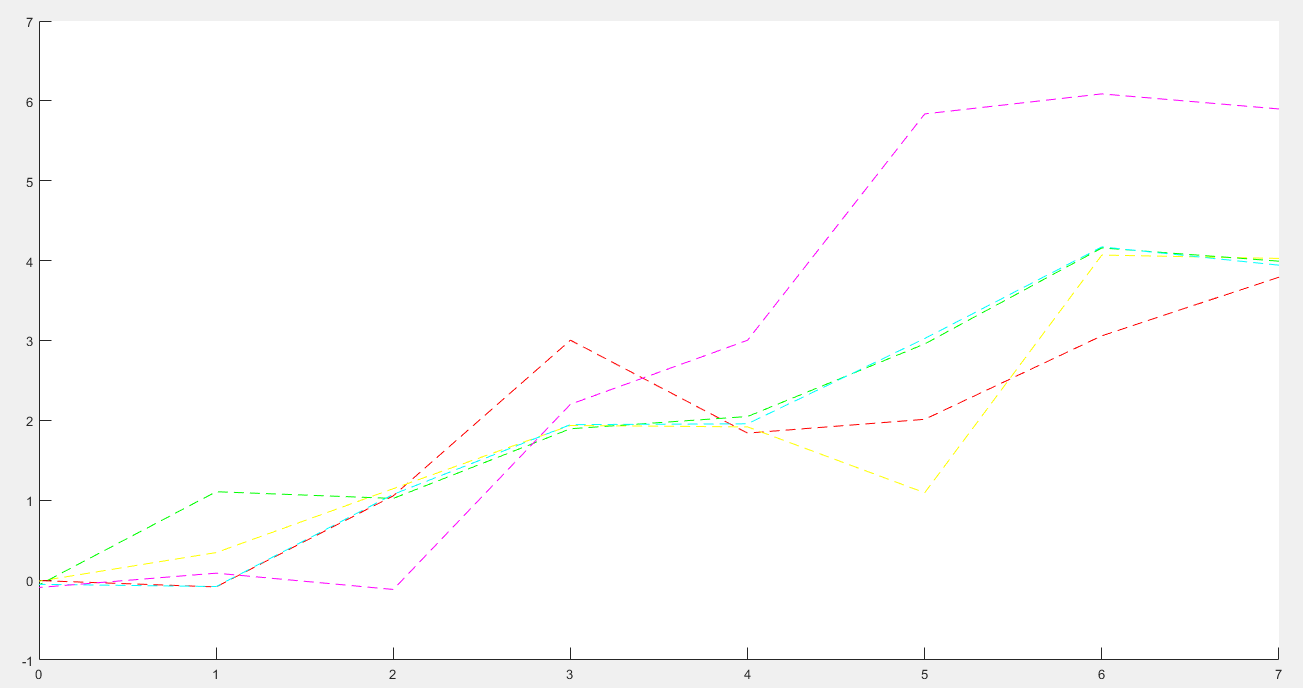
\includegraphics[width=0.95\textwidth]{waterfall}
\captionsetup{justification=centering,margin=1.0 cm}
\caption{SNR graph}
\label{any}
\end{figure}

Красный - Код Хэмминга, Желтый - Код Хэмминга с расчётом синдрома, Зеленый - Циклический Код, Голубой - Код БЧХ, Фиолотовый - Рид-Соломон.
Для Кода Рид-Соломона число ошибок выходит за рамки 4-х бит так как кодирование подразумевает 3 информационных бита емкостью 3 бита каждый.


\vspace{12cm}


\section{Выводы.}

В данной работе нами были получены навыки кодирования и декодирования цифровых сигналов в таких кодах как:
\begin{itemize}
\item Код Хэмминга
\item Циклический код
\item Код БЧХ
\item Код Рида-Соломона
\end{itemize}
Для сравнения Код Хэмминга просто устроен и может быть рассчитан и применён вручную, на листке бумаги, однако он способен исправлять лишь одну ошибку. Код Рида-Соломона может исправлять две ошибки, однако более сложен и может работать с десятичными числами.

\end{document}
